\subsection{Caso d'uso UC5: Gestione profilo utente}

\label{UC5}
\begin{figure}[h]
	\centering
	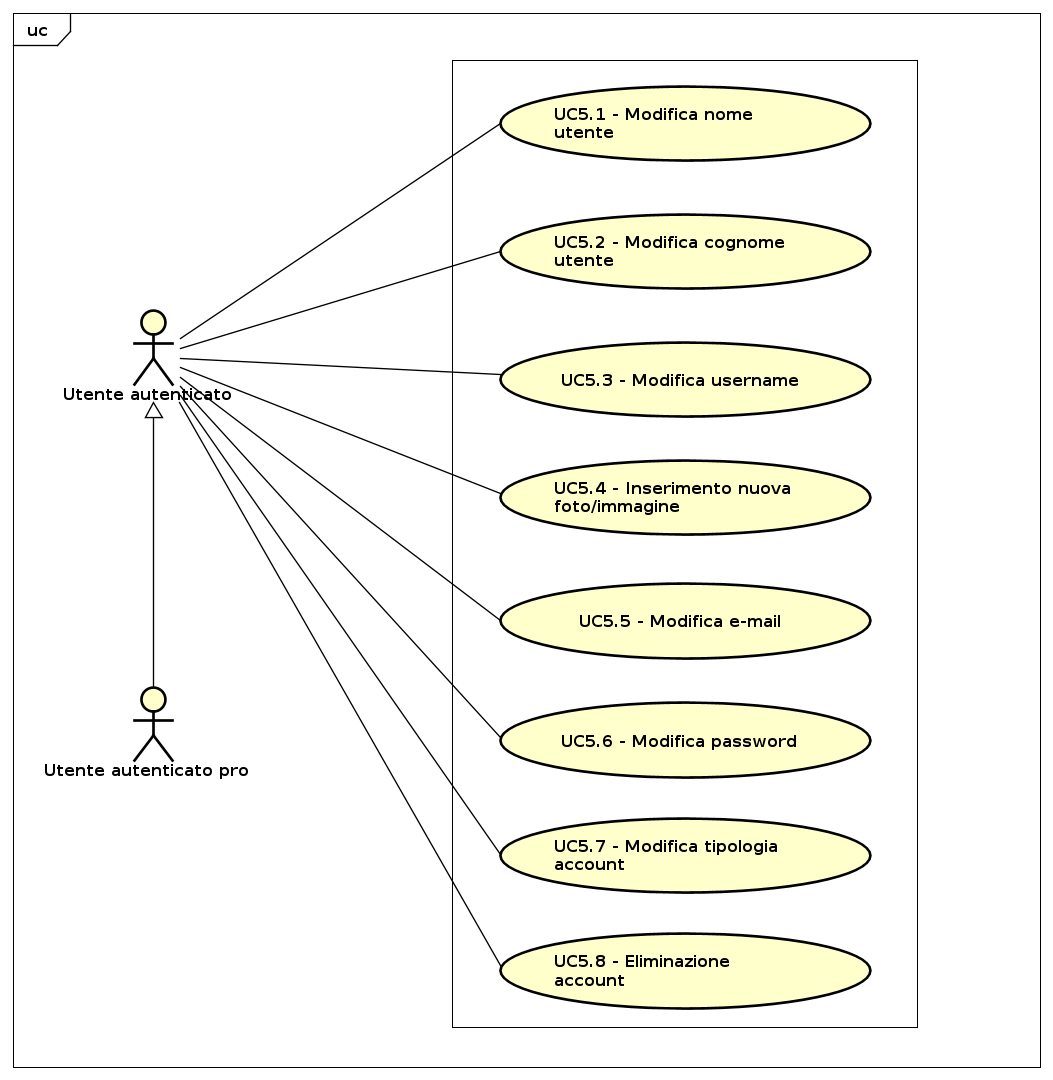
\includegraphics[scale=0.5,keepaspectratio]{UML/UC5.png}
	\caption{UC5: Gestione profilo utente}
\end{figure}
\FloatBarrier
\begin{itemize}
	\item \textbf{Attori}: utente autenticato, utente autenticato pro;
	\item \textbf{Descrizione}: l'attore può visualizzare e modificare i suoi dati personali;
	\item \textbf{Precondizione}: l'attore è entrato nella gestione del proprio profilo utente;
	\item \textbf{Postcondizione}: il sistema ha attuato le modifiche effettuate dall'attore ai propri dati personali;
	\item \textbf{Scenario principale}:
		\begin{enumerate}
			\item L'attore può modificare il proprio nome utente (UC5.1);
			\item L'attore può modificare il proprio cognome utente (UC5.2);
			\item L'attore può modificare il proprio username (UC5.3);
			\item L'attore può inserire una nuova foto/immagine per il proprio profilo utente (UC5.4);
			\item L'attore può modificare la propria e-mail (UC5.5);
			\item L'attore può modificare la propria password (UC5.6);
			\item L'attore può modificare la tipologia del proprio account (UC5.7);
			\item L'attore può eliminare il proprio account (UC5.8).
		\end{enumerate} 
	\item \textbf{Scenari alternativi}: se le operazioni di modifica non vengono confermate il sistema non le rende persistenti e visualizza le funzionalità di gestione del profilo utente. 
\end{itemize}

\subsubsection{Caso d'uso UC5.1: Modifica nome utente}
\label{UC5.1}
\begin{figure}
	\centering
	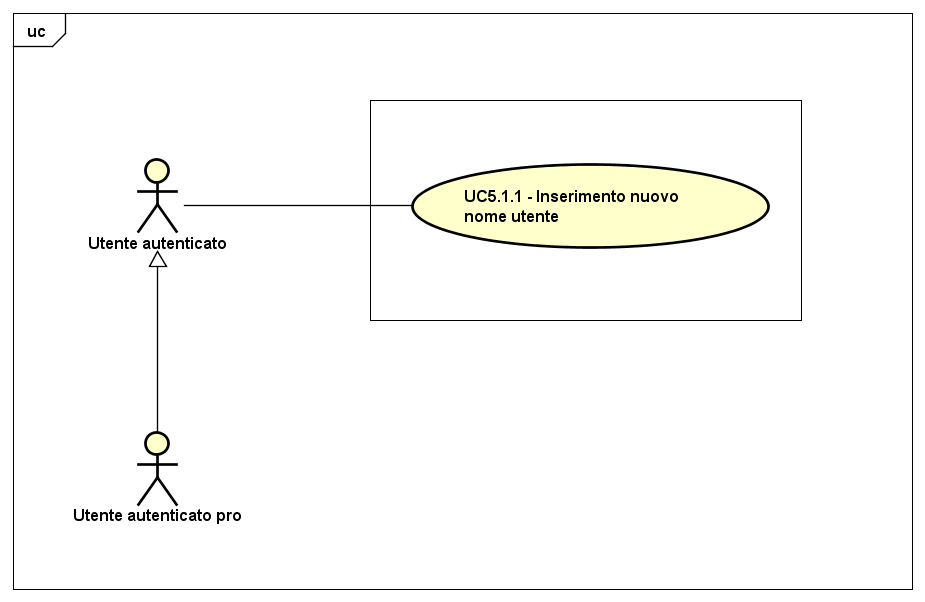
\includegraphics[scale=0.5]{UML/UC5_1.png}
	\caption{UC5.1: Modifica nome utente}
\end{figure}
\begin{itemize}
	\item \textbf{Attori}: utente autenticato, utente autenticato pro;
	\item \textbf{Descrizione}: l'attore può modificare il proprio nome;
	\item \textbf{Precondizione}: l'attore ha selezionato l'opzione modifica nome utente dalla gestione del profilo utente;
	\item \textbf{Postcondizione}: il sistema ha reso persistenti le modifiche al nome utente;
	\item \textbf{Scenario principale}:
		\begin{enumerate}
			\item L'attore può inserire un nuovo nome utente (UC5.1.1);
			\item L'attore può confermare le modifiche al nome utente (UC5.1.2).
		\end{enumerate}
	\item \textbf{Estensione}: l'attore visualizza un messaggio d'errore (UC5.1.3);
	\item \textbf{Scenari alternativi}: l'attore annulla le modifiche e il sistema lo riporta alla schermata di gestione del profilo utente.
\end{itemize}

\subsubsection{Caso d'uso UC5.1.1: Inserimento nuovo nome utente}

\begin{itemize}
	\item \textbf{Attori}: utente autenticato, utente autenticato pro;
	\item \textbf{Descrizione}: l'attore può inserire un nuovo nome utente;
	\item \textbf{Precondizione}: l'attore ha selezionato l'opzione modifica nome utente dalla gestione del profilo utente;
	\item \textbf{Postcondizione}: l'attore ha inserito il nuovo nome utente;
	\item \textbf{Scenario principale}: l'attore inserisce il nuovo nome utente.
\end{itemize}

\subsubsection{Caso d'uso UC5.1.2: Conferma modifiche nome utente}

\begin{itemize}
	\item \textbf{Attori}: utente autenticato, utente autenticato pro;
	\item \textbf{Descrizione}: l'attore può confermare le modifiche al proprio nome utente;
	\item \textbf{Precondizione}: l'attore ha inserito un nuovo nome utente;
	\item \textbf{Postcondizione}: il sistema rende persistenti le modifiche effettuate al nome utente;
	\item \textbf{Scenario principale}: l'attore conferma le modifiche al nome utente.
\end{itemize}

\subsubsection{Caso d'uso UC5.1.3: Visualizzazione errore inserimento nome utente}
\begin{itemize}
	\item \textbf{Attori}: utente autenticato, utente autenticato pro;
	\item \textbf{Descrizione}: l'attore visualizza un messaggio d'errore nell'inserimento del nome utente;
	\item \textbf{Precondizione}: l'attore ha inserito un nome utente non accettato dal sistema;
	\item \textbf{Postcondizione}: il sistema mostra un messaggio di errore;
	\item \textbf{Scenario principale}: l'attore visualizza un messaggio d'errore nell'inserimento del nome utente.
\end{itemize}

\subsubsection{Caso d'uso UC5.2: Modifica cognome utente}
\label{UC5.2}
\begin{figure}[h]
	\centering
	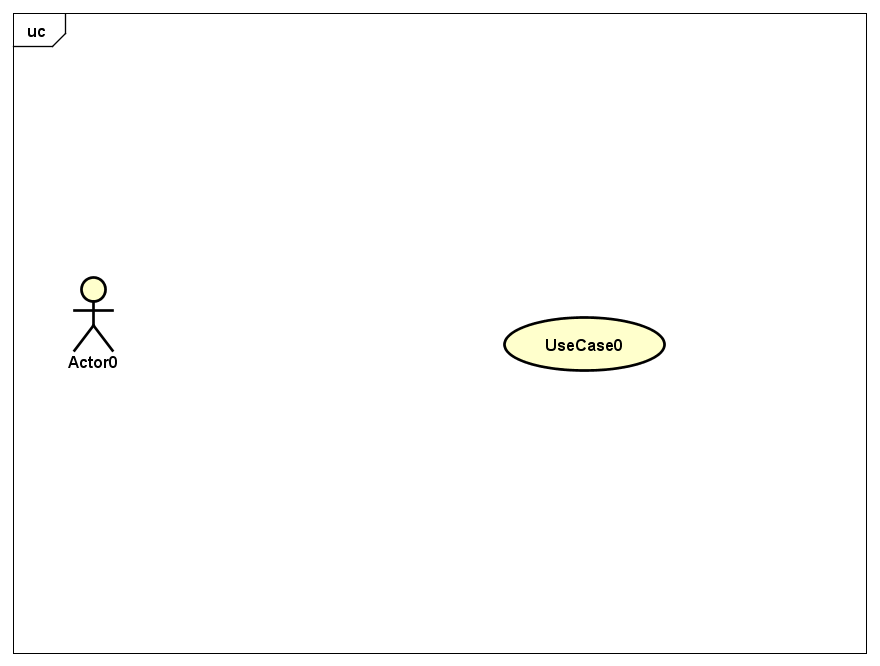
\includegraphics[scale=0.5,keepaspectratio]{UML/UC5_2.png}
	\caption{UC5.2: Modifica cognome utente}
\end{figure}
\begin{itemize}
	\item \textbf{Attori}: utente autenticato, utente autenticato pro;
	\item \textbf{Descrizione}: l'attore può modificare il proprio cognome;
	\item \textbf{Precondizione}: l'attore ha selezionato l'opzione modifica cognome utente dalla gestione del profilo utente; 
	\item \textbf{Postcondizione}: il sistema ha reso persistenti le modifiche al cognome utente;
	\item \textbf{Scenario principale}:
	\begin{enumerate}
		\item L'attore può inserire un nuovo cognome utente (UC5.2.1);
		\item L'attore può confermare le modifiche al cognome utente (UC5.2.2).
	\end{enumerate}
	\item \textbf{Estensione}: l'attore visualizza un messaggio d'errore (UC5.2.3);
	\item \textbf{Scenari alternativi}: l'attore annulla le modifiche e il sistema lo riporta alla schermata di gestione del profilo utente.
\end{itemize}

\subsubsection{Caso d'uso UC5.2.1: Inserimento nuovo cognome utente}

\begin{itemize}
	\item \textbf{Attori}: utente autenticato, utente autenticato pro;
	\item \textbf{Descrizione}: l'attore può inserire un nuovo cognome utente;
	\item \textbf{Precondizione}:  l'attore ha selezionato l'opzione modifica cognome utente dalla gestione del profilo utente; 
	\item \textbf{Postcondizione}:  l'attore ha inserito il nuovo cognome utente;
	\item \textbf{Scenario principale}: l'attore inserisce il nuovo cognome utente.
\end{itemize}

\subsubsection{Caso d'uso UC5.2.2: Conferma modifiche cognome utente}

\begin{itemize}
	\item \textbf{Attori}: utente autenticato, utente autenticato pro;
	\item \textbf{Descrizione}: l'attore può confermare le modifiche al proprio cognome utente;
	\item \textbf{Precondizione}: l'attore ha inserito un nuovo cognome utente;
	\item \textbf{Postcondizione}: il sistema rende persistenti le modifiche effettuate al cognome utente;
	\item \textbf{Scenario principale}: l'attore conferma le modifiche al cognome utente.
\end{itemize}

\subsubsection{Caso d'uso UC5.2.3: Visualizzazione errore inserimento cognome utente}
\begin{itemize}
	\item \textbf{Attori}: utente autenticato, utente autenticato pro;
	\item \textbf{Descrizione}: l'attore visualizza un messaggio d'errore nell'inserimento del cognome utente;
	\item \textbf{Precondizione}: l'attore ha inserito un cognome utente non accettato dal sistema;
	\item \textbf{Postcondizione}: il sistema mostra un messaggio di errore;
	\item \textbf{Scenario principale}: l'attore visualizza un messaggio d'errore nell'inserimento del cognome utente.
\end{itemize}

\subsubsection{Caso d'uso UC5.3: Modifica username}
\label{UC5.3}
\begin{figure}[h]
	\centering
	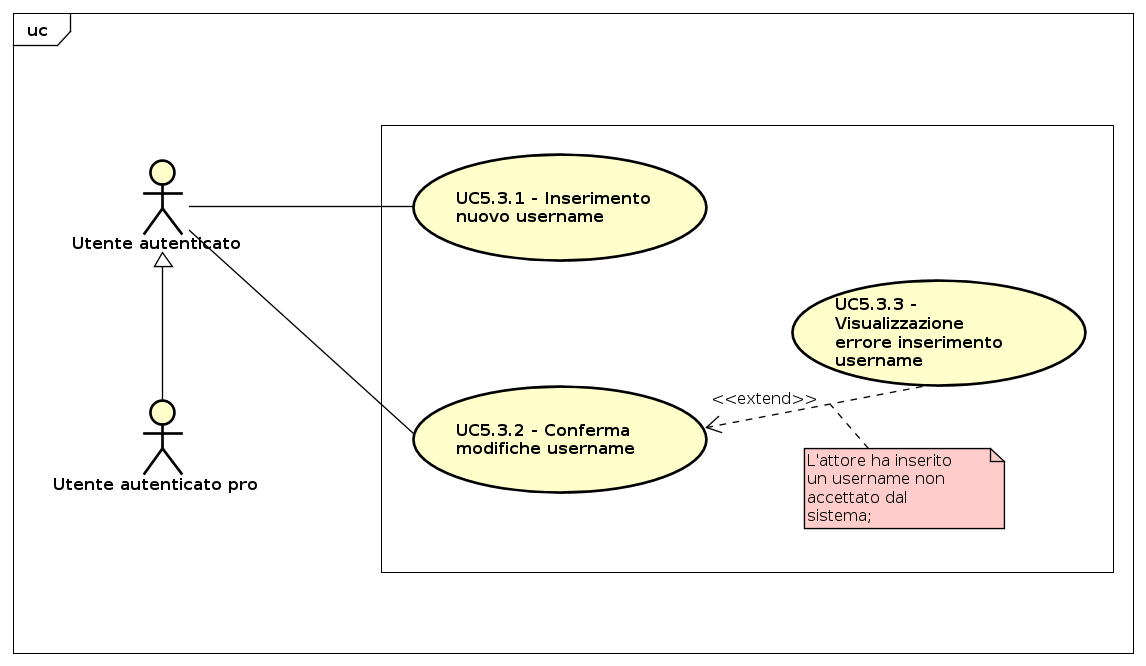
\includegraphics[scale=0.5,keepaspectratio]{UML/UC5_3.png}
	\caption{UC5.3: Modifica username}
\end{figure}
\begin{itemize}
	\item \textbf{Attori}: utente autenticato, utente autenticato pro;
	\item \textbf{Descrizione}: l'attore può modificare il proprio username;
	\item \textbf{Precondizione}: l'attore ha selezionato l'opzione modifica username dalla gestione del profilo utente; 
	\item \textbf{Postcondizione}: il sistema ha reso persistenti le modifiche allo username;
	\item \textbf{Scenario principale}:
	\begin{enumerate}
		\item L'attore può inserire un nuovo username (UC5.3.1);
		\item L'attore può confermare le modifiche allo username (UC5.3.2).
	\end{enumerate}
	\item \textbf{Estensione}: l'attore visualizza un messaggio d'errore (UC5.3.3);
	\item \textbf{Scenari alternativi}: l'attore annulla le modifiche e il sistema lo riporta alla schermata di gestione del profilo utente.
\end{itemize}

\subsubsection{Caso d'uso UC5.3.1: Inserimento nuovo username}

\begin{itemize}
	\item \textbf{Attori}: utente autenticato, utente autenticato pro;
	\item \textbf{Descrizione}: l'attore può inserire un nuovo username;
	\item \textbf{Precondizione}: l'attore ha selezionato l'opzione modifica username dalla gestione del profilo utente; 
	\item \textbf{Postcondizione}: l'attore ha inserito il nuovo username;
	\item \textbf{Scenario principale}: l'attore inserisce il nuovo username.
\end{itemize}

\subsubsection{Caso d'uso UC5.3.2: Conferma modifiche username}

\begin{itemize}
	\item \textbf{Attori}: utente autenticato, utente autenticato pro;
	\item \textbf{Descrizione}: l'attore può confermare le modifiche al proprio username;
	\item \textbf{Precondizione}: l'attore ha inserito un nuovo username;
	\item \textbf{Postcondizione}: il sistema rende persistenti le modifiche effettuate allo username;
	\item \textbf{Scenario principale}: l'attore conferma le modifiche allo username.
\end{itemize}

\subsubsection{Caso d'uso UC5.3.3: Visualizzazione errore inserimento username}
\begin{itemize}
	\item \textbf{Attori}: utente autenticato, utente autenticato pro;
	\item \textbf{Descrizione}: l'attore visualizza un messaggio d'errore nel caso nell'inserimento dell'username;
	\item \textbf{Precondizione}: l'attore ha inserito un username non accettato dal sistema;
	\item \textbf{Postcondizione}: il sistema mostra un messaggio di errore;
	\item \textbf{Scenario principale}: l'attore visualizza un messaggio d'errore nell'inserimento del nome utente.
\end{itemize}

\subsubsection{Caso d'uso UC5.4: Inserimento foto/immagine}
\label{UC5.4}
\begin{figure}[h]
	\centering
	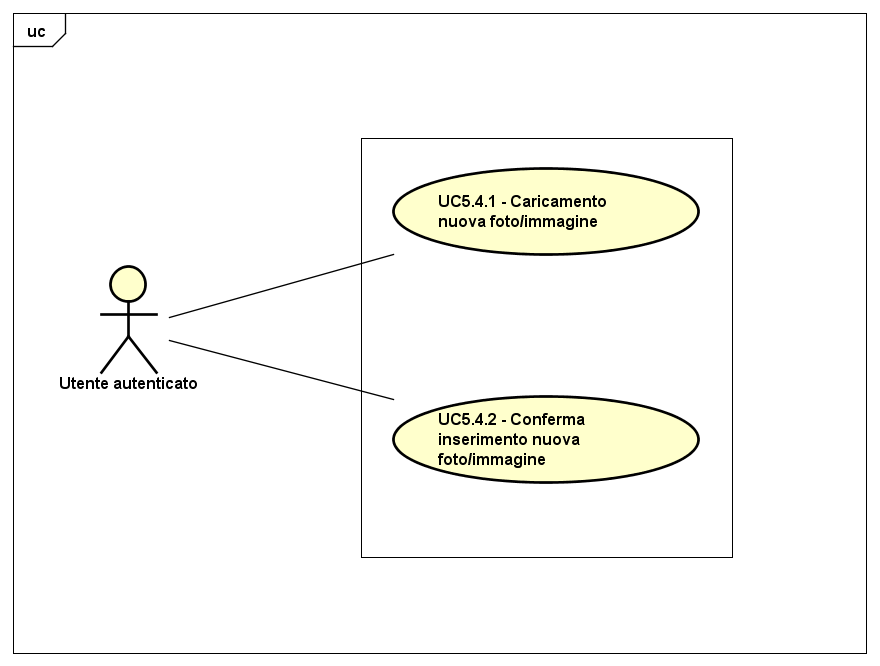
\includegraphics[scale=0.5,keepaspectratio]{UML/UC5_4.png}
	\caption{UC5.4: Inserimento foto/immagine}
\end{figure}
\begin{itemize}
	\item \textbf{Attori}: utente autenticato, utente autenticato pro;
	\item \textbf{Descrizione}: l'attore può inserire una foto/immagine per il proprio profilo utente;
	\item \textbf{Precondizione}: l'attore ha selezionato l'opzione inserimento foto/immagine dalla gestione del profilo utente; 
	\item \textbf{Postcondizione}: il sistema ha allegato la nuova foto/immagine al profilo utente;
	\item \textbf{Scenario principale}:
	\begin{enumerate}
		\item L'attore può caricare una nuova foto/immagine nel sistema (UC5.4.1);
		\item L'attore può confermare l'inserimento della nuova foto/immagine (UC5.4.2).
	\end{enumerate}
	\item \textbf{Estensione}: l'attore visualizza un messaggio d'errore (UC5.4.3);
	\item \textbf{Scenari alternativi}: l'attore annulla l'inserimento e il sistema lo riporta alla schermata di gestione del profilo utente.
\end{itemize}

\subsubsection{Caso d'uso UC5.4.1: Caricamento foto/immagine}

\begin{itemize}
	\item \textbf{Attori}: utente autenticato, utente autenticato pro;
	\item \textbf{Descrizione}: l'attore può caricare una nuova foto/immagine;
	\item \textbf{Precondizione}: l'attore ha selezionato l'opzione inserimento foto/immagine dalla gestione del profilo utente;  
	\item \textbf{Postcondizione}: l'attore ha caricato una nuova foto/immagine;
	\item \textbf{Scenario principale}: l'attore carica una nuova foto/immagine.
\end{itemize}

\subsubsection{Caso d'uso UC5.4.2: Conferma caricamento foto/immagine}

\begin{itemize}
	\item \textbf{Attori}: utente autenticato, utente autenticato pro;
	\item \textbf{Descrizione}: l'attore può confermare il caricamento della nuova foto/immagine;
	\item \textbf{Precondizione}: l'attore ha caricato una nuova foto/immagine;
	\item \textbf{Postcondizione}: il sistema allega la nuova foto/immagine al profilo utente;
	\item \textbf{Scenario principale}: l'attore conferma il caricamento della nuova foto/immagine.
\end{itemize}

\subsubsection{Caso d'uso UC5.4.3: Visualizzazione errore inserimento foto/immagine}
\begin{itemize}
	\item \textbf{Attori}: utente autenticato, utente autenticato pro;
	\item \textbf{Descrizione}: l'attore visualizza un messaggio d'errore nell'inserimento di una foto/immagine;
	\item \textbf{Precondizione}: l'attore ha inserito una foto/immagine non accettata dal sistema;
	\item \textbf{Postcondizione}: il sistema mostra un messaggio di errore;
	\item \textbf{Scenario principale}: l'attore visualizza un messaggio d'errore nell'inserimento di una foto/immagine.
\end{itemize}

\subsubsection{Caso d'uso UC5.5: Modifica e-mail}
\label{UC5.5}
\begin{figure}[h]
	\centering
	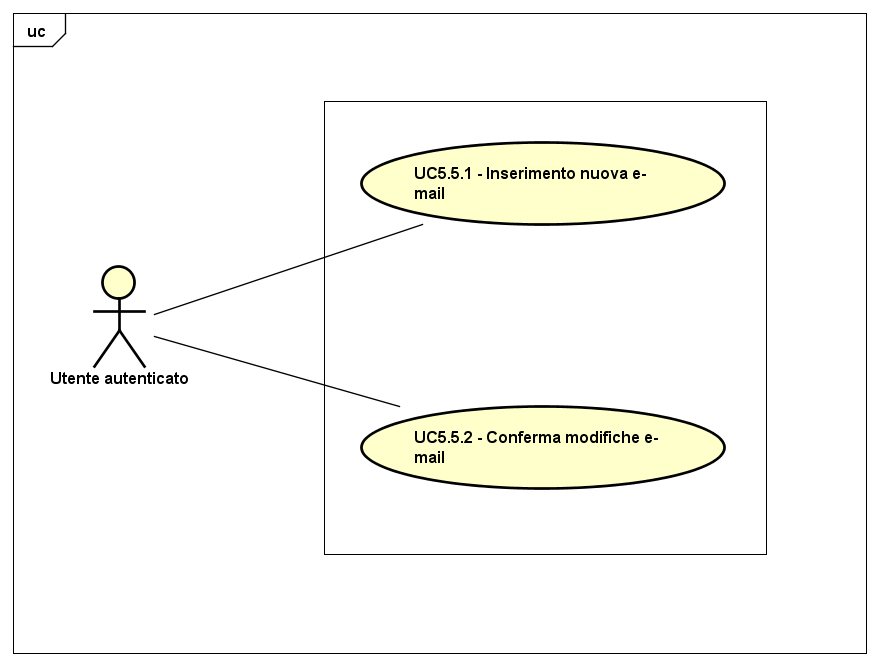
\includegraphics[scale=0.5,keepaspectratio]{UML/UC5_5.png}
	\caption{UC5.5: Modifica e-mail}
\end{figure}

\begin{itemize}
	\item \textbf{Attori}: utente autenticato, utente autenticato pro;
	\item \textbf{Descrizione}: l'attore può modificare il proprio indirizzo di posta elettronica inserendone uno nuovo;
	\item \textbf{Precondizione}:  l'attore ha selezionato l'opzione modifica e-mail dalla gestione del profilo utente; 
	\item \textbf{Postcondizione}: il sistema ha reso persistenti le modifiche all'indirizzo di posta elettronica;
	\item \textbf{Scenario principale}:
		\begin{enumerate}
			\item L'attore può inserire un nuovo indirizzo di posta elettronica (UC5.5.1);
			\item L'attore può confermare le modifiche al proprio indirizzo di posta elettronica (UC5.5.2).
		\end{enumerate}
		\item \textbf{Estensione}: l'attore visualizza un messaggio d'errore (UC5.5.3);
	\item \textbf{Scenari alternativi}: l'attore annulla le modifiche e il sistema lo riporta alla schermata di gestione del profilo utente.
\end{itemize}

\subsubsection{Caso d'uso UC5.5.1: Inserimento nuova e-mail}

\begin{itemize}
	\item \textbf{Attori}: utente autenticato, utente autenticato pro;
	\item \textbf{Descrizione}: l'attore può inserire un nuovo indirizzo di posta elettronica;
	\item \textbf{Precondizione}:  l'attore ha selezionato l'opzione modifica e-mail dalla gestione del profilo utente;
	\item \textbf{Postcondizione}: l'attore ha inserito un nuovo indirizzo di posta elettronica;
	\item \textbf{Scenario principale}: l'attore inserisce un nuovo indirizzo di posta elettronica.
\end{itemize}

\subsubsection{Caso d'uso UC5.5.2: Conferma modifiche e-mail}

\begin{itemize}
	\item \textbf{Attori}: utente autenticato, utente autenticato pro;
	\item \textbf{Descrizione}: l'attore può confermare le modifiche al proprio indirizzo di posta elettronica;
	\item \textbf{Precondizione}: l'attore ha inserito un nuovo indirizzo di posta elettronica;
	\item \textbf{Postcondizione}: il sistema rende persistenti le modifiche effettuate all'indirizzo di posta elettronica;
	\item \textbf{Scenario principale}: l'attore conferma le modifiche all'indirizzo di posta elettronica.
\end{itemize}

 \subsubsection{Caso d'uso UC5.5.3: Visualizzazione errore inserimento e-mail}
 \begin{itemize}
 	\item \textbf{Attori}: utente autenticato, utente autenticato pro;
 	\item \textbf{Descrizione}: l'attore visualizza un messaggio d'errore nell'inserimento dell'indirizzo di posta elettronica;
 	\item \textbf{Precondizione}: l'attore ha inserito un indirizzo di posta elettronica non accettato dal sistema;
 	\item \textbf{Postcondizione}: il sistema mostra un messaggio di errore;
 	\item \textbf{Scenario principale}: l'attore visualizza un messaggio d'errore nell'inserimento dell'indirizzo di posta elettronica.
 \end{itemize}

\subsubsection{Caso d'uso UC5.6: Modifica password}
\label{UC5.6}
\begin{figure}[h]
	\centering
	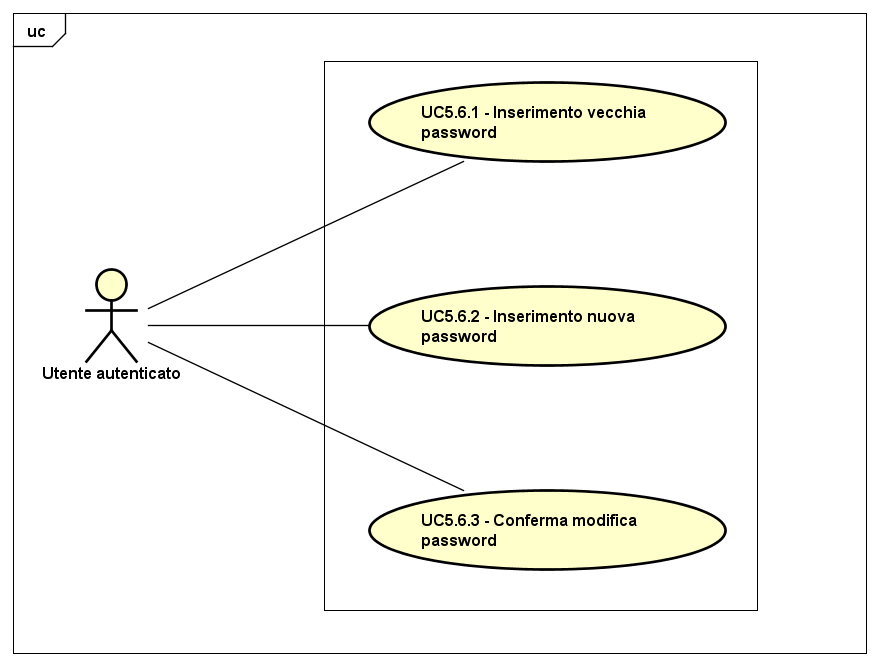
\includegraphics[scale=0.5,keepaspectratio]{UML/UC5_6.png}
	\caption{UC5.6: Modifica password}
\end{figure}

\begin{itemize}
	\item \textbf{Attori}: utente autenticato, utente autenticato pro;
	\item \textbf{Descrizione}: l'attore può modificare la propria password inserendone una nuova;
	\item \textbf{Precondizione}:  l'attore ha selezionato l'opzione modifica password dalla gestione del profilo utente;
	\item \textbf{Postcondizione}: il sistema ha reso persistenti le modifiche alla propria password;
	\item \textbf{Scenario principale}:
	\begin{enumerate}
		\item L'attore può inserire la propria vecchia password (UC5.6.1);
		\item L'attore può inserire una nuova password (UC5.6.2);
		\item L'attore può confermare la modifica della password (UC5.6.3).
	\end{enumerate}
	\item \textbf{Estensione}: l'attore visualizza un messaggio d'errore (UC5.6.4);
	\item \textbf{Scenari alternativi}: l'attore annulla le modifiche e il sistema lo riporta alla schermata di gestione del profilo utente.
\end{itemize}

\subsubsection{Caso d'uso UC5.6.1: Inserimento vecchia password}

\begin{itemize}
	\item \textbf{Attori}: utente autenticato, utente autenticato pro;
	\item \textbf{Descrizione}: l'attore può inserire la vecchia password;
	\item \textbf{Precondizione}:  l'attore ha selezionato l'opzione modifica e-mail dalla gestione del profilo utente;
	\item \textbf{Postcondizione}: l'attore ha inserito la vecchia password;
	\item \textbf{Scenario principale}: l'attore inserisce la vecchia password.
\end{itemize}

\subsubsection{Caso d'uso UC5.6.2: Inserimento nuova password}

\begin{itemize}
	\item \textbf{Attori}: utente autenticato, utente autenticato pro;
	\item \textbf{Descrizione}: l'attore può inserire la nuova password;
	\item \textbf{Precondizione}: l'attore ha inserito la vecchia password;
	\item \textbf{Postcondizione}: l'attore inserisce la nuova password;
	\item \textbf{Scenario principale}: l'attore inserisce la nuova password.
\end{itemize}

\subsubsection{Caso d'uso UC5.6.3: Inserimento conferma nuova password}

\begin{itemize}
	\item \textbf{Attori}: utente autenticato, utente autenticato pro;
	\item \textbf{Descrizione}: l'attore può inserire la nuova password nuovamente;
	\item \textbf{Precondizione}: l'attore ha inserito la nuova password;
	\item \textbf{Postcondizione}: l'attore inserisce nuovamente la nuova password;
	\item \textbf{Scenario principale}: l'attore inserisce nuovamente la nuova password.
\end{itemize}

\subsubsection{Caso d'uso UC5.6.4: Conferma modifica password}

\begin{itemize}
	\item \textbf{Attori}: utente autenticato, utente autenticato pro;
	\item \textbf{Descrizione}: l'attore può confermare le modifiche alla password effettuate;
	\item \textbf{Precondizione}: l'attore ha inserito tutti i campi richiesti per il cambio di password;
	\item \textbf{Postcondizione}: il sistema rende persistenti le modifiche effettuate alla password;
	\item \textbf{Scenario principale}: l'attore conferma le modifiche alla password effettuate.
\end{itemize}

\subsubsection{Caso d'uso UC5.6.5: Visualizzazione errore inserimento password}
\begin{itemize}
	\item \textbf{Attori}: utente autenticato, utente autenticato pro;
	\item \textbf{Descrizione}: l'attore visualizza un messaggio d'errore nell'inserimento della password;
	\item \textbf{Precondizione}: l'attore ha inserito una password non accettata dal sistema;
	\item \textbf{Postcondizione}: il sistema mostra un messaggio di errore;
	\item \textbf{Scenario principale}: l'attore visualizza un messaggio d'errore  nell'inserimento della password.
\end{itemize}

\subsubsection{Caso d'uso UC5.7: Cambio tipologia account}
\label{UC5.7}
\begin{figure}[h]
	\centering
	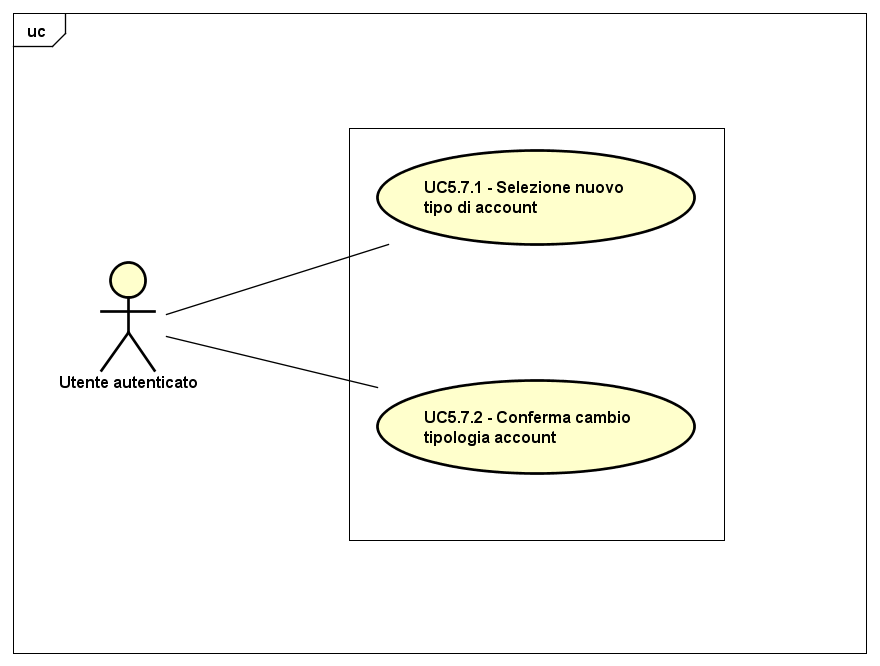
\includegraphics[scale=0.5,keepaspectratio]{UML/UC5_7.png}
	\caption{UC5.7: Cambio tipologia account}
\end{figure}

\begin{itemize}
	\item \textbf{Attori}: utente autenticato, utente autenticato pro;
	\item \textbf{Descrizione}: l'attore può cambiare la tipologia del proprio account; 
	\item \textbf{Precondizione}:  l'attore ha selezionato l'opzione cambio tipologia di account dalla gestione del profilo utente;
	\item \textbf{Postcondizione}: il sistema ha cambiato la tipologia dell'account;
	\item \textbf{Scenario principale}:
	\begin{enumerate}
		\item L'attore può selezionare il nuovo tipo di account a cui passare (UC5.7.1)
		\item L'attore può confermare il cambio di tipologia del proprio account (UC5.7.2).
	\end{enumerate}
	\item \textbf{Scenari alternativi}: l'attore annulla le modifiche e il sistema lo riporta alla schermata di gestione del profilo utente.
\end{itemize}

\subsubsection{Caso d'uso UC5.7.1: Selezione tipologia account}

\begin{itemize}
	\item \textbf{Attori}: utente autenticato, utente autenticato pro;
	\item \textbf{Descrizione}: l'attore può selezionare una nuova tipologia di account a cui passare;
	\item \textbf{Precondizione}: l'attore ha selezionato l'opzione cambio tipologia di account dalla gestione del profilo utente;
	\item \textbf{Postcondizione}: l'attore ha selezionato  una nuova tipologia di account;
	\item \textbf{Scenario principale}: l'attore seleziona una tipologia di account a cui passare.
\end{itemize}

\subsubsection{Caso d'uso UC5.7.2: Conferma cambio tipologia account}

\begin{itemize}
	\item \textbf{Attori}: utente autenticato, utente autenticato pro;
	\item \textbf{Descrizione}: l'attore può confermare la tipologia di account a cui passare;
	\item \textbf{Precondizione}: l'attore ha selezionato la nuova tipologia di account;
	\item \textbf{Postcondizione}: il sistema cambia la tipologia dell'account;
	\item \textbf{Scenario principale}: l'attore conferma la nuova tipologia di account a cui passare.
\end{itemize}

\subsubsection{Caso d'uso UC5.8: Eliminazione account}
\label{UC5.8}
\begin{figure}[h]
	\centering
	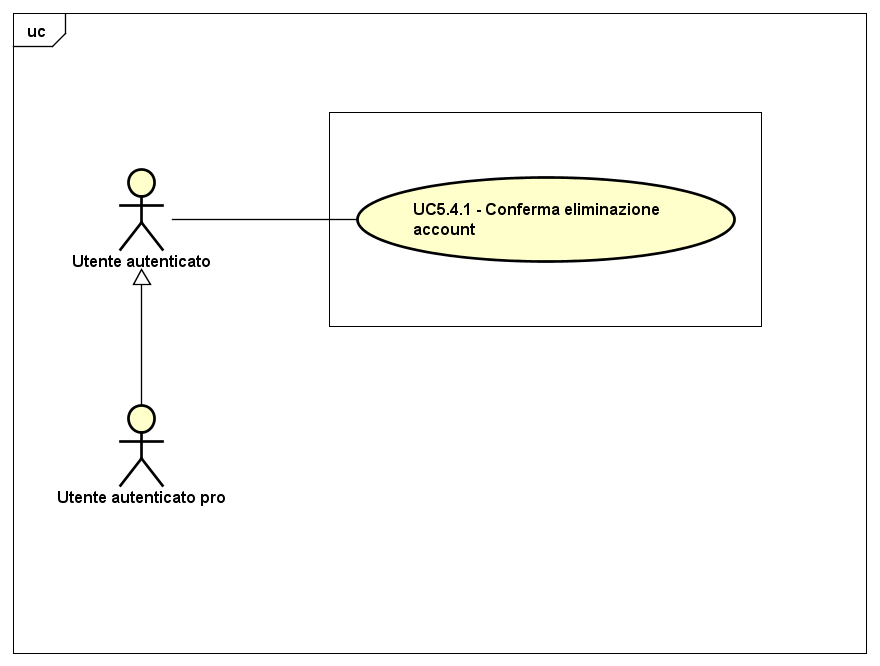
\includegraphics[scale=0.5,keepaspectratio]{UML/UC5_8.png}
	\caption{UC5.8: Eliminazione account}
\end{figure}

\begin{itemize}
	\item \textbf{Attori}: utente autenticato, utente autenticato pro;
	\item \textbf{Descrizione}: l'attore può eliminare il proprio account dal sistema; l'eliminazione dell'account comporta la cancellazione dei propri dati dal sistema; 
	\item \textbf{Precondizione}: l'attore ha selezionato l'opzione di eliminazione account;
	\item \textbf{Postcondizione}: il sistema ha eliminato in maniera persistente l'account e tutti i relativi dati;
	\item \textbf{Scenario principale}:
		\begin{enumerate}
			\item L'utente può confermare l'eliminazione del proprio account e dei relativi dati personali (UC5.8.1).
		\end{enumerate}
		\item \textbf{Scenari alternativi}: l'attore annulla l'eliminazione dell'account e il sistema lo riporta alla schermata di gestione del profilo utente.
\end{itemize}

\subsubsection{Caso d'uso UC5.8.1: Conferma eliminazione account}

\begin{itemize}
	\item \textbf{Attori}: utente autenticato, utente autenticato pro;
	\item \textbf{Descrizione}: l'attore può confermare la cancellazione del proprio account e dei relativi dati dal sistema;
	\item \textbf{Precondizione}: l'attore ha selezionato l'opzione di eliminazione account;
	\item \textbf{Postcondizione}: il sistema ha eliminato l'account dell'attore richiedente e tutti i relativi dati;
	\item \textbf{Scenario principale}: l'attore conferma l'eliminazione del proprio account.
\end{itemize}